\emph{Note:} The schematic  for the  LT3471's circuit  is located  in appendix
\ref{appendix:lt3741:circuit} on page \pageref{appendix:lt3741:circuit}. It is
intended  to be  folded out  while reading  this section  of the  report. This
allows for convenient cross-referencing between  the circuit schematic and the
text without needing to insert multiple  copies of the schematic or constantly
scrolling back and forth through the report.

The most important reasons we chose  the LT3741 to regulate the output voltage
are as follows:

\begin{itemize}
    \item \textbf{Proven Technologies.}
        Switch-mode  regulators have  been around  for decades  and have  been
        perfected by many engineers.
    \item \textbf{Voltage and current requirements.}
        The device is specified to output voltage levels between \SI{0}{\volt}
        and  \SI{24}{\volt} and  current  levels  between \SI{0}{\ampere}  and
        \SI{3.5}{\ampere}.   Further, the  ripple voltage  is specified  to be
        $\le\SI{300}{\milli\volt}$  and the  ripple  current  is specified  to
        be  $\le\SI{100}{\milli\ampere}$. The  LT3741  fulfills all  of  these
        requirements.
    \item \textbf{The importance of power absorption.}
        Most switch-mode regulators are only  able to \emph{supply} power, but
        are  incapable of  \emph{absorbing} power. Because  our device  may be
        connected in series  (or parallel) with other power  supplies, it must
        have  the ability  to absorb  power  (which is  the case  if, it  were
        connected to a  voltage source outputting a higher  voltage level than
        our own).
    \item \textbf{Control inputs.}
        The LT3741  has dedicated  input control pins  to change  directly the
        output  current. This simplifies  the  design  because no  complicated
        additional circuitry is required.
\end{itemize}

%\begin{figure}[th!]
%    \center
%    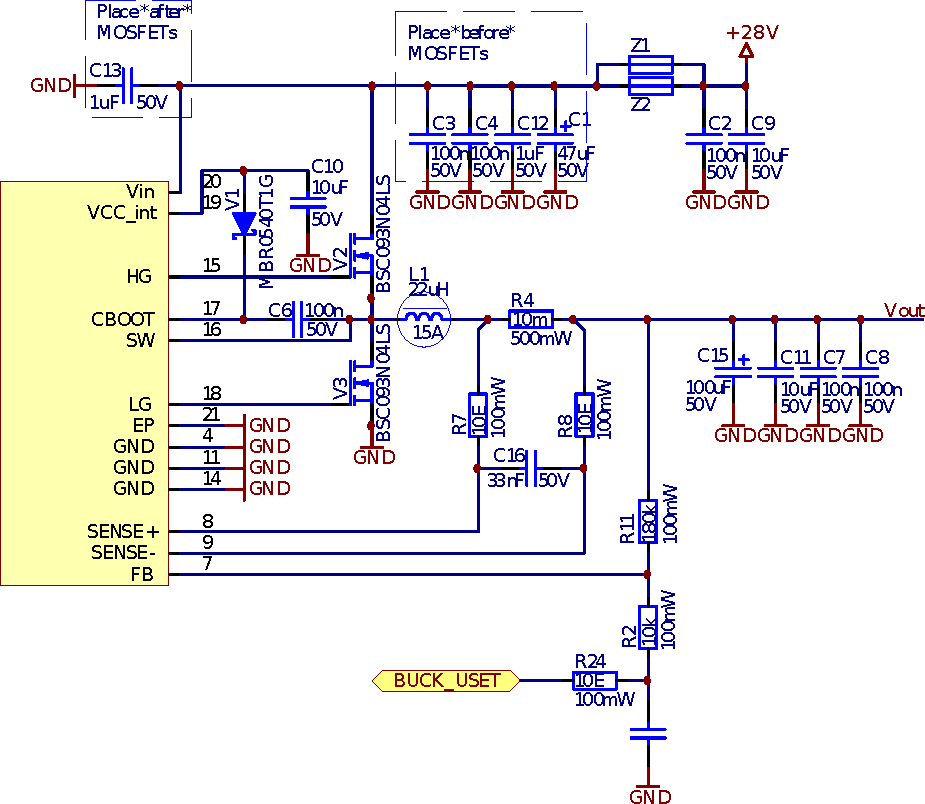
\includegraphics[width=.67\textwidth]{images/circuit/buck.pdf}
%    %\caption{Herzst\"uck des Projektes: Aufbau des LT3741 CVCC Synchronwandler}
%    \caption{The device's heart: Overview over circuit for the LT3741 CCVC synchronous converter.}
%    \label{fig:circuit:buck}
%\end{figure}

Figure \ref{fig:circuit:buck} on the fold-out (see \emph{Note} above) presents
an overview  for the LT3741's  circuit, parts of  which are discussed  in more
detail in  the following paragraphs:  Bypass  capacitors, switching frequency,
inductors, MOSFETs and measuring output current and output voltage.


% **************************************************************************** %
\subsubsection{Bypass Capacitors}
% **************************************************************************** %

The LT3741 is powered by the \SI{28}{\volt}  rail, which can be seen in Figure
\ref{fig:circuit:buck} in the  top right. The switching of  the MOSFETs causes
the LT13741  to consume high amounts  of power in short  bursts. This leads to
the LT3741  feeding high  frequency disturbance  back into  the \SI{28}{\volt}
rail, which  could lead  to disturbances  in the  rest of  the circuit  if not
handled correctly.  As a countermeasure,  a multitude of different ceramic and
electrolytic bypass  capacitors in parallel  are used.  Additionally,  we used
ferrite beads, placed  in series with the supply to  absorb any high frequency
feedback.


% **************************************************************************** %
\subsubsection{Switching Frequency}
% **************************************************************************** %

There is a trade-off when  selecting the switching frequency $f_S$. The higher
$f_S$,  the lower  the output  ripple voltage  will be. However,  the LT3741's
power  consumption will  also increase  due to  switching losses.   Generally,
$f_S$ is to be maximised to reduce ripple.

Because so  much depends  on $f_S$,  it is more  convenient to  determine this
value empirically through simulations. The  most suitable value was determined
to be $f_S \approx\SI{800}{\kilo\hertz}$. In the remaining calculations, $f_S$
is assumed to be \SI{1}{\mega\hertz} to allow for some leeway.

%A specific  resistor on one  of the LT3741's inputs  is used to  configure the
%switching frequency $f_S$.


% **************************************************************************** %
\subsubsection{Inductor Selection}
\label{subsubsec:lt3741:inductors}
% **************************************************************************** %

The   size    of   the    inductor   $L_1$,    as   illustrated    in   Figure
\ref{fig:circuit:buck}  on  the fold-out,  was  calculated  using the  formula
below:

\begin{equation}
    L_1 = \left( \frac{V_{in} \cdot V_{out} - V_{out}^2}{0.3 \cdot f_S \cdot I_O \cdot V_{in}} \right) = \SI{6}{\micro\henry}
    \label{eq:circuit:buck:inductor}
\end{equation}

where  $V_{in}$ equals  the  input voltage  \SI{28}{\volt},  $V_{out}$ is  the
output voltage  at peak  power (which exists  at $V_{out}  = \SI{14}{\volt}$),
$f_S$ is the switching frequency  \SI{1}{\mega\hertz} and $I_O$ is the maximum
output  current, assumed  to be  $I_O  = \SI{5}{\ampere}$,  allowing for  some
additional leeway.   A larger  inductor of  $L_1 =  \SI{22}{\micro\henry}$ was
selected to further decrease ripple current.

In addition to the inductance, the maximum current rating, DCR, and saturation
current are also important factors to consider. The inductor's peak current is
calculated using
\begin{equation}
    I_{L_{1_{peak}}} = I_O + \left( \frac{V_{in} \cdot V_{out} - V_{out}^2}{2 \cdot f_S \cdot L_1 \cdot V_{in}} \right) = \SI{5.2}{\ampere}
    \label{eq:circuit:buck:inductor_peak}
\end{equation}

Where  $V_{in}$ equals  the  input voltage  \SI{28}{\volt},  $V_{out}$ is  the
output voltage  at peak  power (which exists  at $V_{out}  = \SI{14}{\volt}$),
$f_S$ is  the switching frequency  \SI{1}{\mega\hertz}, $L_1$ is the  value of
the selected inductor (\SI{22}{\micro\henry}) and  $I_O$ is the maximum output
current, assumed  to be  $I_O =  \SI{5}{\ampere}$.  The  inductor's saturation
current  was  sized  $1.2$  times  higher than  the  peak  current. With  this
defined,  a list  of  possible inductors  could be  compiled,  shown in  Table
\ref{tab:circuit:buck:inductor} in  appendix \ref{appendix:inductors}  on page
\pageref{appendix:inductors}.   We chose  the \emph{732-4237-1-ND}  because it
has the lowest DCR (direct current resistance) of the models listed.


% **************************************************************************** %
\subsubsection{MOSFET Selection}
\label{subsubsec:lt3741:mosfets}
% **************************************************************************** %

In contrast to a non-synchronous  regulator, our design uses two complementary
MOSFETs $V_2$ and $V_3$ (in the middle of Figure \ref{fig:circuit:buck} on the
fold-out) , whereby $V_3$ acts as  an active replacement for the free wheeling
diode  typically found  in  non-synchronous designs. As  mentioned earlier,  a
crucial feature of  this device is the ability to  \emph{absorb} power.  $V_3$
does this by regulating current in the opposite direction through the inductor
$L_1$.

When  selecting  switching  MOSFETs,  the  following  parameters are critical in
determining the best devices for a given application: $Q_G$ (Total Gate Charge),
$R_{DS_{(on)}}$ (On-Resistance), $Q_{GD}$ (Gate to Drain Charge), $Q_{GS}$ (Gate
to Source  Charge),  $R_G$ (Gate Resistance), $V_{GS}$ (gate-to-source voltage),
$V_{DS}$  (drain-to-source-voltage),  $I_{D_{max}}$  (peak  drain  current)  and
$V_{GS_{THR}}$ (gate threshold voltage).

The     maximum     drain     current     is     equal     to     the     peak
inductor    current    $I_{L_{1_{peak}}}$    as   calculated    in    equation
\ref{eq:circuit:buck:inductor_peak}: $I_{D_{max}}    =   I_{L_{1_{peak}}}    =
\SI{5.2}{\ampere}$

%\begin{equation}
%    I_{D_{max}} = I_{L_{1_{peak}}} = I_O + \left(\frac{V_{in}\cdot V_{out} - V_{out}^2}{2\cdot f_S \cdot L_1 \cdot V_{in}}\right) = \SI{5.2}{\ampere}
%    \label{eq:circuit:buck:mosfet_id}
%\end{equation}

The maximum  drain-to-source voltage $V_{DS}$  must be greater than  the input
voltage  $V_{in}  =  \SI{28}{\volt}$,  including  transients,   otherwise  the
MOSFETs will be damaged. MOSFETs with $V_{DS} = \SI{40}{\volt}$ were therefore
selected.

The  signals driving  the  gates of  the  MOSFETs have  a  maximum voltage  of
\SI{5}{\volt}  with  respect to  the  source.   During start-up  and  recovery
conditions, the gate drive signals  may be as low as \SI{3}{\volt}. Therefore,
to  ensure that  the  LT3741  recovers properly,  the  maximum gate  threshold
voltage should  be less than  \SI{2}{\volt}. For a robust design,  the maximum
gate-to-source voltage $V_{GS}$ should be greater than \SI{7}{\volt}.

Power losses in  the MOSFETs are related to  the on-resistance $R_{DS{(on)}}$,
the  transition losses  related to  the gate  resistance $R_G$,  gate-to-drain
capacitance  $Q_{GD}$  and  gate-to-source  capacitance  $Q_{GS}$. Power  loss
to  the  on-resistance  is  an  Ohmic  loss,  $I^2  R_{DS_{(on)}}$. The  power
loss  in  the  high  side  MOSFET $V_2$  can  be  approximated  with  equation
\ref{eq:circuit:buck:mosfet_ploss}.

\begin{multline}
    P_{LOSS} = (\textrm{ohmic loss}) + (\textrm{transission loss}) \\
             \approx \left( I_O^2 \cdot R_{DS_{(on)}} \cdot \rho_T \right)
                    + \left( \frac{V_{in} \cdot I_O}{\SI{5}{\volt}} \cdot \left(Q_{GD} + Q_{GS} \right) \cdot \left( 2 \cdot R_G + R_{PU} + R_{PD} \right) \cdot f_S \right) \\
    \label{eq:circuit:buck:mosfet_ploss}
\end{multline}
whereby   $\rho_T$   is  a   temperature-dependant   term   of  the   MOSFET's
on-resistance.  Using \SI{70}{\degree C} as the maximum operating temperature,
$\rho_T$  roughly equals  $1.3$.  $R_{PD}$  and $R_{PU}$  are the  LT3741 high
side  gate  driver  output   impedances,  \SI{1.3}{\ohm}  and  \SI{2.3}{\ohm},
respectively.

Driving the gates also causes power loss in switching MOSFETs.  The total gate
charge, $Q_G$, must be charged and discharged switch each switching cycle. The
power is  lost to the internal  LDO within the  LT3741. The power lost  to the
charging of the gates is:
\begin{equation}
    P_{LOSS\_LDO} \approx \left( (V_{in} - \SI{5}{\volt} \right) \cdot \left( Q_{GLG} + Q_{GHG} \right) \cdot f_S
    \label{eq:circuit:buck:switching_loss}
\end{equation}
whereby $G_{GLG}$ is the  low side gate charge and $Q_{GHG}$  is the high side
gate charge.

Table  \ref{tab:circuit:buck:mosfet}  in  appendix  \ref{appendix:mosfets}  on
page  \pageref{appendix:mosfets} lists  possible MOSFETs  that meet  the above
constraints.  For  each one  the power  losses $P_{LOSS}$  and $P_{LOSS\_LDO}$
were calculated. The  MOSFET which  ended up  being selected  is not  the best
model, but it is a lot cheaper than the best fit and has better documentation.


% **************************************************************************** %
\subsubsection{Measurement of Output Voltage and Output Current}
\label{subsubsec:lt3741:feedback}
% **************************************************************************** %

\begin{minipage}{0.5\textwidth}
    The LT3741  is both voltage  regulated and current  regulated. The voltage
    divider  $R_{11}  \parallel  R_2$  (Figure  \ref{fig:circuit:buck:uset}  )
    allows for  the measurement of  the output  voltage, and a  shunt resistor
    $R_4$ allows  for the exact monitoring  of the current going  through coil
    $L_1$. The value  for resistor $R_4$ (fold-out  overview schematic, Figure
    \ref{fig:circuit:buck}) was chosen so that the maximum outoing current can
    be \SI{5}{\ampere}.

    Monitoring the  current is extremely  important for  a setup in  which the
    outgoing  voltage can  be constantly  changing. It allows  to predict  the
    behavior  of  the output  voltage,  thus  enabling  the device  to  better
    suppress spikes in  output voltage and spikes in the  current through coil
    $L_1$ (Figure \ref{fig:circuit:buck} on fold-out).

    Furthermore,  a  controller   regulated  by  current  can   also  be  used
    as  a  constant  current  source. This  property  is  of  importance  when
    the  operating  point   is  in  the  steeper  part  of   the  PV  module's
    I-V-curve  (where   small  changes   in  voltage   can  lead   to  drastic
    changes  in current,  see section  \ref{subsec:regimplementation} on  page
    \pageref{subsec:regimplementation}).

\end{minipage}
\begin{minipage}{0.5\textwidth}
    \center
    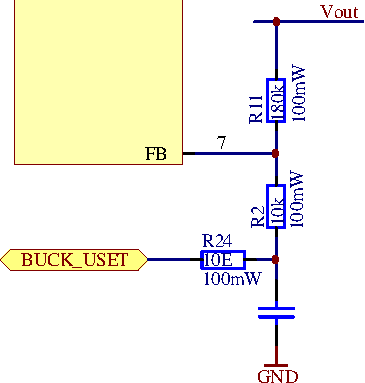
\includegraphics[width=.85\textwidth]{images/circuit/buck-uset.pdf}
    %\captionof{figure}{Regulation of output voltage by changing the reference voltage in the feedback loop via an analog reference voltage between \SI{0}{\volt} and \SI{1.21}{\volt}}
    \captionof{figure}{Circuit for regulating output voltage by changing reference voltage via $BUCK\_USET$ from the first DAC}
    \label{fig:circuit:buck:uset}
\end{minipage}

\begin{minipage}{.4\textwidth}
    The  values for  the feedback  resistors  $R_2$ and  $R_{11}$ were  chosen
    according to formula  \ref{eq:circuit:buck:feedback_resistors} so that the
    output voltage does not exceed \SI{23}{\volt}.
\end{minipage}
\begin{minipage}{.6\textwidth}
    \begin{equation}
        V_{out} = \SI{1.21}{\volt} \left( 1 + \frac{R_{11}}{R_2} \right)
        \label{eq:circuit:buck:feedback_resistors}
    \end{equation}
\end{minipage}

\begin{minipage}{.40\textwidth}
    By  increasing  $BUCK\_USET$  in formula  \ref{eq:circuit:buck:uset},  the
    outgoing  voltage can  then be  modified as  needed.  $BUCK\_USET$  is the
    analog voltage  coming from the  first DAC. The associated circuit  can be
    found in Figure \ref{fig:circuit:buck:uset}.
\end{minipage}
\begin{minipage}{.60\textwidth}
    \begin{equation}
        V_{out} = (\SI{1.21}{\volt} - BUCK\_USET) \cdot \frac{R_{11} + R_2}{R_2}
        \label{eq:circuit:buck:uset}
    \end{equation}
\end{minipage}


\begin{minipage}{.50\textwidth}
    In a manner analogous to regulating the output voltage, the maximum output
    current can  also be  controlled.  By applying  an analog  voltage between
    \SI{0}{\volt}  and \SI{1.5}{\volt}  at  input \code{CTRL1}  of the  LT3741
    controller,  the maximum  average  current going  through  coil $L_1$  and
    therefore the maximum output current can be directly controlled.

    The     corresponding    circuit     can     be     found    in     Figure
    \ref{fig:circuit:buck:iset}.  The maximum average  output current $I_o$ is
    calculated using equation \ref{eq:circuit:buck:output_current}.

    For  this, $V_{CTRL1}$  is the  analog reference  voltage coming  from the
    second DAC and  $R_4$ is the shunt  resistor (\SI{10}{\milli\ohm}, visible
    on the fold-out in Figure \ref{fig:circuit:buck}).

\end{minipage}
\begin{minipage}{.50\textwidth}
    \center
    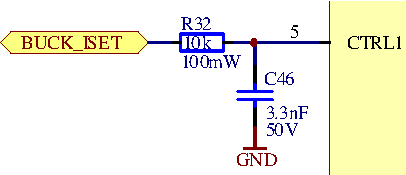
\includegraphics[width=.9\textwidth]{images/circuit/buck-iset.pdf}
    \captionof{figure}{Setting the maximum output current via reference voltage between \SI{0}{\volt} and \SI{1.5}{\volt}}
    \label{fig:circuit:buck:iset}
    \begin{equation}
        I_o = \frac{V_{CTRL1}}{30 \cdot R_4}
        \label{eq:circuit:buck:output_current}
    \end{equation}
\end{minipage}


\begin{minipage}{.50\textwidth}
    For  the  microcontroller  to  generate  appropriate  reference  voltages,
    it  needs  to   measure  both  output  voltage   and  output  current. The
    output    voltage   is    measured    with   the    circuit   in    Figure
    \ref{fig:circuit:buck:umeas}. The  values   for  resistors   $R_{12}$  and
    $R_{15}$  are such  that  voltage  $BUCK\_UMEAS$ is  scaled  to the  range
    between \SI{0}{\volt} and \SI{1.5}{\volt}.

    The  output   current  is  measured  differentially   via  shunt  resistor
    $R_5$. The    corresponding   circuit    can    be    seeen   in    Figure
    \ref{fig:circuit:buck:imeas}.

\end{minipage}
\begin{minipage}{.50\textwidth}
    \center
    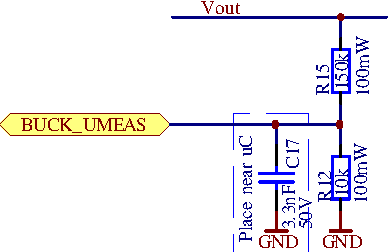
\includegraphics[width=.8\textwidth]{images/circuit/buck-umeas.pdf}
    \captionof{figure}{Measuring output voltage}
    \label{fig:circuit:buck:umeas}
\end{minipage}

\begin{figure}[th!]
    \center
    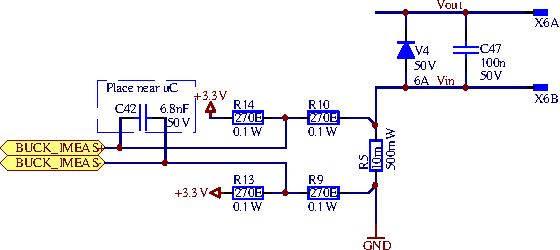
\includegraphics[width=.85\textwidth]{images/circuit/buck-imeas.pdf}
    \caption{Measuring output current}
    \label{fig:circuit:buck:imeas}
\end{figure}

\begin{minipage}{.50\textwidth}
A  particular problem  for this  measurement  is that  resistors $R_{10}$  and
$R_{14}$ cause a  bias current to flow through the  shunt resistor $R_5$, thus
leading  to an  offset $V_{offset}$  of the  measured voltage  over $R_5$,  as
calculated by equation \ref{eq:circuit:buck:shunt_offset}.
\end{minipage}
\begin{minipage}{.50\textwidth}
    \begin{equation}
        V_{offset} = \frac{ \SI{3.3}{\volt} \cdot R_5 }{ R_{14} + R_{10} + R_5 }
        \label{eq:circuit:buck:shunt_offset}
    \end{equation}
\end{minipage}

\begin{minipage}{.50\textwidth}
    Since  the  ADC  has  a  resolution   of  12  bits  and  a  reference  voltage
    of   \SI{3.3}{\volt},   one  voltage   increment   amounts   to  $V_{step}   =
    \frac{\SI{3.3}{\volt}}{2^{12}} = \SI{806}{\micro\volt}$

    Resistors $R_9$,  $R_{10}$, $R_{13}$  and $R_{14}$ should  be as  small as
    possible in order to reduce disturbances  in the traces, while at the same
    time being large enough for $V_{offset}$ to be smaller than $V_{step}$. In
    order for the ADC's holding time not to be too long (which happens roughly
    at $\geq \SI{5}{\kilo\ohm}$), they should however also not be too large.

    Thus, we can now  solve for the four resistor values,  as seen in on the right.
\end{minipage}
\begin{minipage}{.50\textwidth}

    %Equations \ref{eq:circuit:buck:shunt_offset} \ref{eq:circuit:buck:adc_step} can now
    %be solved for the four resistor values:

    \begin{align*}
                              V_{step} &\geq V_{offset} \\
        \frac{\SI{3.3}{\volt}}{2^{12}} &\geq \SI{3.3}{\volt} \cdot \frac{R_5}{R_x + R_5} \\
                      \frac{1}{2^{12}} &\geq \frac{R_5}{R_x + R_5} \\
                                   R_x &\geq \left( 2^{12} - 1 \right) \cdot R_5 \\
        \label{eq:solvethings}
    \end{align*}
    \hspace*{2em}whereby $\frac{R_x}{2} =  R_{9} = R_{10} = R_{13} =  R_{14}$.
\end{minipage}

This yields as its result $\frac{R_x}{2} \approx \SI{22}{\ohm}$.


\begin{minipage}{.50\textwidth}
    A  further  limitation,  especially  for  smaller  resistors,  is  not  to
    dissipate  too  much  power. For  this   reason,  the  resistors  will  be
    dimensioned  slightly   higher  at  \SI{270}{\ohm}. Thus,   the  resulting
    dissipated  power for  all  four resistors  is  calcualted using  equation
    \ref{eq:P_loss}.
\end{minipage}
\begin{minipage}{.50\textwidth}
    \begin{equation} \label{eq:P_loss}
        P_{loss} \approx \frac{\left(\SI{3.3}{\volt}\right)^2}{2\cdot \SI{270}{\ohm}} \approx \SI{20}{\milli\watt}
    \end{equation}
\end{minipage}

The measured  voltage at the  shunt resistor is comparatively  small. For this
reason, we use the microcontroller's integrated pre-amplifier (PGA), which can
attain a gain  of up to factor  64. The amplified signal is then  passed on to
the internal differential ADC.


% **************************************************************************** %
\subsubsection{Output}
% **************************************************************************** %

Two  banana  plugs  $X_{6A}$  and  $X_{6B}$  provide  the  connection  to  the
output  voltage,  while  reverse  voltage protection  is  achieved  via  diode
$V_4$.   (Figure \label{fig:circuit:output}).   An external  reference voltage
of  \SI{1.5}{\volt}  is  used to  ensure  that  the  ADCs  and DACs  can  make
accurate  measurements and  can  be used  over their  full  range (see  figure
\ref{fig:circuit:vref}).

\begin{minipage}{.50\textwidth}
    \center
    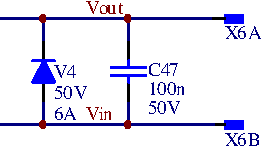
\includegraphics[width=.9\textwidth]{images/circuit/output-connectors.pdf}
    \captionof{figure}{Reverse voltage protection at output}
    \label{fig:circuit:output}
\end{minipage}
\begin{minipage}{.50\textwidth}
    \center
    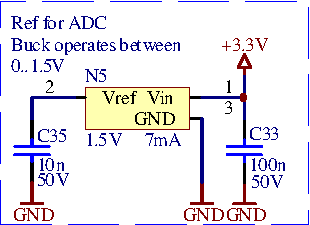
\includegraphics[width=.8\textwidth]{images/circuit/vref.pdf}
    \captionof{figure}{%
        \SI{1.5}{\volt} reference voltage for full-range operation of DACs
        and DACs
    }
    \label{fig:circuit:vref}
\end{minipage}



% **************************************************************************** %
\subsubsection{Enable and Under-Voltage Lockout circuit}
% **************************************************************************** %

\begin{minipage}{0.5\textwidth}
    The  LT3741's  \emph{Enable}   input  is  enabled  and   disabled  by  the
    microcontroller's $BUCK\_EN$ signal  on one hand, on the other  hand it is
    can  be  forcibly  disabled  in  hardware  when  the  \SI{28}{\volt}  rail
    drops below  \SI{25}{\volt}. This allows for a  controlled and predictable
    behavior of  the LT3741  during power-on and  power-off. The corresponding
    circuit can be found in Figure \ref{fig:circuit:uvlo}.

    In  case of  under-voltage, $N_6$  switches  on and  the transistor  $V_6$
    starts to  conduct, thus  pulling the  \emph{Enable} input  to \emph{Low}.
    Voltage $BUCK\_UVLO$ triggers an interrupt in the microcontroller.
\end{minipage}
\begin{minipage}{0.5\textwidth}
    \center
    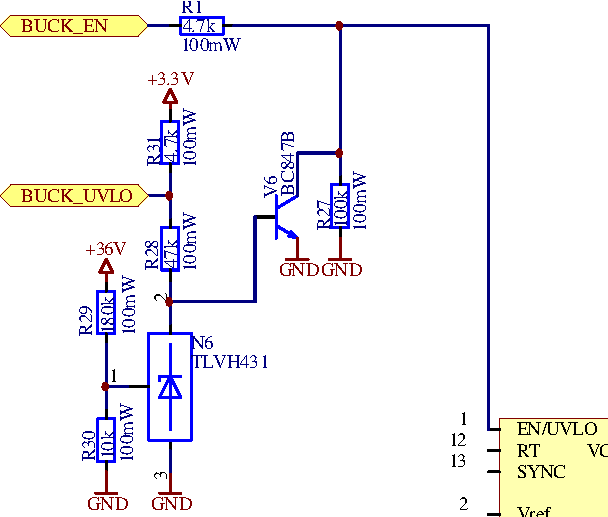
\includegraphics[width=.8\textwidth]{images/circuit/uvlo.pdf}
    \captionof{figure}{Under-Voltage Lock-Out (UVLO) allows for controlled power-on and power-off of the controller}
    \label{fig:circuit:uvlo}
\end{minipage}


